% Options for packages loaded elsewhere
\PassOptionsToPackage{unicode}{hyperref}
\PassOptionsToPackage{hyphens}{url}
%
\documentclass[
]{book}
\usepackage{amsmath,amssymb}
\usepackage{lmodern}
\usepackage{iftex}
\ifPDFTeX
  \usepackage[T1]{fontenc}
  \usepackage[utf8]{inputenc}
  \usepackage{textcomp} % provide euro and other symbols
\else % if luatex or xetex
  \usepackage{unicode-math}
  \defaultfontfeatures{Scale=MatchLowercase}
  \defaultfontfeatures[\rmfamily]{Ligatures=TeX,Scale=1}
\fi
% Use upquote if available, for straight quotes in verbatim environments
\IfFileExists{upquote.sty}{\usepackage{upquote}}{}
\IfFileExists{microtype.sty}{% use microtype if available
  \usepackage[]{microtype}
  \UseMicrotypeSet[protrusion]{basicmath} % disable protrusion for tt fonts
}{}
\makeatletter
\@ifundefined{KOMAClassName}{% if non-KOMA class
  \IfFileExists{parskip.sty}{%
    \usepackage{parskip}
  }{% else
    \setlength{\parindent}{0pt}
    \setlength{\parskip}{6pt plus 2pt minus 1pt}}
}{% if KOMA class
  \KOMAoptions{parskip=half}}
\makeatother
\usepackage{xcolor}
\usepackage{color}
\usepackage{fancyvrb}
\newcommand{\VerbBar}{|}
\newcommand{\VERB}{\Verb[commandchars=\\\{\}]}
\DefineVerbatimEnvironment{Highlighting}{Verbatim}{commandchars=\\\{\}}
% Add ',fontsize=\small' for more characters per line
\usepackage{framed}
\definecolor{shadecolor}{RGB}{248,248,248}
\newenvironment{Shaded}{\begin{snugshade}}{\end{snugshade}}
\newcommand{\AlertTok}[1]{\textcolor[rgb]{0.94,0.16,0.16}{#1}}
\newcommand{\AnnotationTok}[1]{\textcolor[rgb]{0.56,0.35,0.01}{\textbf{\textit{#1}}}}
\newcommand{\AttributeTok}[1]{\textcolor[rgb]{0.77,0.63,0.00}{#1}}
\newcommand{\BaseNTok}[1]{\textcolor[rgb]{0.00,0.00,0.81}{#1}}
\newcommand{\BuiltInTok}[1]{#1}
\newcommand{\CharTok}[1]{\textcolor[rgb]{0.31,0.60,0.02}{#1}}
\newcommand{\CommentTok}[1]{\textcolor[rgb]{0.56,0.35,0.01}{\textit{#1}}}
\newcommand{\CommentVarTok}[1]{\textcolor[rgb]{0.56,0.35,0.01}{\textbf{\textit{#1}}}}
\newcommand{\ConstantTok}[1]{\textcolor[rgb]{0.00,0.00,0.00}{#1}}
\newcommand{\ControlFlowTok}[1]{\textcolor[rgb]{0.13,0.29,0.53}{\textbf{#1}}}
\newcommand{\DataTypeTok}[1]{\textcolor[rgb]{0.13,0.29,0.53}{#1}}
\newcommand{\DecValTok}[1]{\textcolor[rgb]{0.00,0.00,0.81}{#1}}
\newcommand{\DocumentationTok}[1]{\textcolor[rgb]{0.56,0.35,0.01}{\textbf{\textit{#1}}}}
\newcommand{\ErrorTok}[1]{\textcolor[rgb]{0.64,0.00,0.00}{\textbf{#1}}}
\newcommand{\ExtensionTok}[1]{#1}
\newcommand{\FloatTok}[1]{\textcolor[rgb]{0.00,0.00,0.81}{#1}}
\newcommand{\FunctionTok}[1]{\textcolor[rgb]{0.00,0.00,0.00}{#1}}
\newcommand{\ImportTok}[1]{#1}
\newcommand{\InformationTok}[1]{\textcolor[rgb]{0.56,0.35,0.01}{\textbf{\textit{#1}}}}
\newcommand{\KeywordTok}[1]{\textcolor[rgb]{0.13,0.29,0.53}{\textbf{#1}}}
\newcommand{\NormalTok}[1]{#1}
\newcommand{\OperatorTok}[1]{\textcolor[rgb]{0.81,0.36,0.00}{\textbf{#1}}}
\newcommand{\OtherTok}[1]{\textcolor[rgb]{0.56,0.35,0.01}{#1}}
\newcommand{\PreprocessorTok}[1]{\textcolor[rgb]{0.56,0.35,0.01}{\textit{#1}}}
\newcommand{\RegionMarkerTok}[1]{#1}
\newcommand{\SpecialCharTok}[1]{\textcolor[rgb]{0.00,0.00,0.00}{#1}}
\newcommand{\SpecialStringTok}[1]{\textcolor[rgb]{0.31,0.60,0.02}{#1}}
\newcommand{\StringTok}[1]{\textcolor[rgb]{0.31,0.60,0.02}{#1}}
\newcommand{\VariableTok}[1]{\textcolor[rgb]{0.00,0.00,0.00}{#1}}
\newcommand{\VerbatimStringTok}[1]{\textcolor[rgb]{0.31,0.60,0.02}{#1}}
\newcommand{\WarningTok}[1]{\textcolor[rgb]{0.56,0.35,0.01}{\textbf{\textit{#1}}}}
\usepackage{longtable,booktabs,array}
\usepackage{calc} % for calculating minipage widths
% Correct order of tables after \paragraph or \subparagraph
\usepackage{etoolbox}
\makeatletter
\patchcmd\longtable{\par}{\if@noskipsec\mbox{}\fi\par}{}{}
\makeatother
% Allow footnotes in longtable head/foot
\IfFileExists{footnotehyper.sty}{\usepackage{footnotehyper}}{\usepackage{footnote}}
\makesavenoteenv{longtable}
\usepackage{graphicx}
\makeatletter
\def\maxwidth{\ifdim\Gin@nat@width>\linewidth\linewidth\else\Gin@nat@width\fi}
\def\maxheight{\ifdim\Gin@nat@height>\textheight\textheight\else\Gin@nat@height\fi}
\makeatother
% Scale images if necessary, so that they will not overflow the page
% margins by default, and it is still possible to overwrite the defaults
% using explicit options in \includegraphics[width, height, ...]{}
\setkeys{Gin}{width=\maxwidth,height=\maxheight,keepaspectratio}
% Set default figure placement to htbp
\makeatletter
\def\fps@figure{htbp}
\makeatother
\setlength{\emergencystretch}{3em} % prevent overfull lines
\providecommand{\tightlist}{%
  \setlength{\itemsep}{0pt}\setlength{\parskip}{0pt}}
\setcounter{secnumdepth}{5}
\usepackage{booktabs}
\usepackage{longtable}
\usepackage[bf,singlelinecheck=off]{caption}
\captionsetup[table]{labelsep=space}
\captionsetup[figure]{labelsep=space}
\usepackage[scale=.7]{sourcecodepro}

% not in https://github.com/yihui/bookdown-crc/blob/master/latex/preamble.tex
\usepackage{tabu}
\usepackage{graphicx}
%%%

\usepackage{framed,color}
\definecolor{shadecolor}{RGB}{255,255,255}
\definecolor{shadecolor2}{RGB}{236,240,249}

\renewcommand{\textfraction}{0.05}
\renewcommand{\topfraction}{0.8}
\renewcommand{\bottomfraction}{0.8}
\renewcommand{\floatpagefraction}{0.75}

\renewenvironment{quote}{\begin{VF}}{\end{VF}}
\usepackage{hyperref}
\let\oldhref\href
% \renewcommand{\href}[2]{#2\footnote{\url{#1}}}

% code blocks style (e.g., background)
\makeatletter
\newenvironment{kframe}{%
\medskip{}
\setlength{\fboxsep}{.8em}
 \def\at@end@of@kframe{}%
 \ifinner\ifhmode%
  \def\at@end@of@kframe{\end{minipage}}%
  \begin{minipage}{\columnwidth}%
 \fi\fi%
 \def\FrameCommand##1{\hskip\@totalleftmargin \hskip-\fboxsep
 \colorbox{shadecolor}{##1}\hskip-\fboxsep
     % There is no \\@totalrightmargin, so:
     \hskip-\linewidth \hskip-\@totalleftmargin \hskip\columnwidth}%
 \MakeFramed {\advance\hsize-\width
   \@totalleftmargin\z@ \linewidth\hsize
   \@setminipage}}%
 {\par\unskip\endMakeFramed%
 \at@end@of@kframe}
\makeatother

\renewenvironment{Shaded}{\begin{kframe}}{\end{kframe}}

% text blocks style (e.g., background)
\makeatletter
\newenvironment{kframe2}{%
\medskip{}
\setlength{\fboxsep}{.8em}
 \def\at@end@of@kframe2{}%
 \ifinner\ifhmode%
  \def\at@end@of@kframe2{\end{minipage}}%
  \begin{minipage}{\columnwidth}%
 \fi\fi%
 \def\FrameCommand##1{\hskip\@totalleftmargin \hskip-\fboxsep
 \colorbox{shadecolor2}{##1}\hskip-\fboxsep
     % There is no \\@totalrightmargin, so:
     \hskip-\linewidth \hskip-\@totalleftmargin \hskip\columnwidth}%
 \MakeFramed {\advance\hsize-\width
   \@totalleftmargin\z@ \linewidth\hsize
   \@setminipage}}%
 {\par\unskip\endMakeFramed%
 \at@end@of@kframe2}
\makeatother


% not in https://github.com/yihui/bookdown-crc/blob/master/latex/preamble.tex
\newenvironment{rmdblock}[1]
  {
  \begin{itemize}
  \renewcommand{\labelitemi}{
    \raisebox{-.7\height}[0pt][0pt]{
      {\setkeys{Gin}{width=3em,keepaspectratio}\includegraphics{images/#1}}
    }
  }
  \setlength{\fboxsep}{1em}
  \begin{kframe2}
  \item
  }
  {
  \end{kframe2}
  \end{itemize}
  }
\newenvironment{rmdnote}
  {\begin{rmdblock}{globe}}
  {\end{rmdblock}}
%%%

\usepackage{makeidx}
\makeindex

\urlstyle{tt}

\usepackage{amsthm}
\makeatletter
\def\thm@space@setup{%
  \thm@preskip=8pt plus 2pt minus 4pt
  \thm@postskip=\thm@preskip
}
\makeatother

\frontmatter
\ifLuaTeX
  \usepackage{selnolig}  % disable illegal ligatures
\fi
\usepackage[]{natbib}
\bibliographystyle{apalike}
\IfFileExists{bookmark.sty}{\usepackage{bookmark}}{\usepackage{hyperref}}
\IfFileExists{xurl.sty}{\usepackage{xurl}}{} % add URL line breaks if available
\urlstyle{same} % disable monospaced font for URLs
\hypersetup{
  pdftitle={Catálogo DataMet},
  hidelinks,
  pdfcreator={LaTeX via pandoc}}

\title{Catálogo DataMet}
\author{}
\date{\vspace{-2.5em}}

\usepackage{amsthm}
\newtheorem{theorem}{Theorem}[chapter]
\newtheorem{lemma}{Lemma}[chapter]
\newtheorem{corollary}{Corollary}[chapter]
\newtheorem{proposition}{Proposition}[chapter]
\newtheorem{conjecture}{Conjecture}[chapter]
\theoremstyle{definition}
\newtheorem{definition}{Definition}[chapter]
\theoremstyle{definition}
\newtheorem{example}{Example}[chapter]
\theoremstyle{definition}
\newtheorem{exercise}{Exercise}[chapter]
\theoremstyle{definition}
\newtheorem{hypothesis}{Hypothesis}[chapter]
\theoremstyle{remark}
\newtheorem*{remark}{Remark}
\newtheorem*{solution}{Solution}
\begin{document}
\maketitle

{
\setcounter{tocdepth}{1}
\tableofcontents
}
\hypertarget{descripciuxf3n}{%
\chapter*{Descripción}\label{descripciuxf3n}}
\addcontentsline{toc}{chapter}{Descripción}

Ante el objetivo de desarrollar una plataforma de datos interoperables para la toma de decisiones para la Región Metropolitana, el presente catálogo de datos se presenta como un primer acercamiento y sistematización de toda la información necesaria para conformar dicha plataforma.

Este catálogo se construyó a partir de un marco normativo internacional y de gobernabilidad de los datos, tomando como punto de partida el marco institucional nacional. Así, la elaboración de un catastro de información espacial y no espacial, homologado a través de una serie de mecanismos (como por ejemplo los escenarios creados conjuntamente con el Gobierno Regional para definir la utilidad de los datos), permitió la consolidación de un catálogo de datos interoperables.

El desarrollo de un Catálogo de Datos se basa en estándares que permitan catastrar los datos espaciales y no espaciales, como también, conocer sus alcances y el estado de la información, de forma de que estos puedan ser consultados por distintas instituciones y actores, y así, asegurar su interoperabilidad.

Por medio de la \textbf{\texttt{Norma\ ISO\ 19.110}} se define una metodología para catalogar Objetos Geográficos. Los elementos que componen un catálogo de features presentan una organización que conlleva características de orden y jerarquía, como se presenta en la siguiente Figura.

\textbf{Render book}

\begin{Shaded}
\begin{Highlighting}[]
\CommentTok{\# bookdown::render\_book()}
\CommentTok{\# bookdown::serve\_book()}
\end{Highlighting}
\end{Shaded}

\hypertarget{uxe1mbito-informaciuxf3n-base}{%
\chapter{Ámbito: Información Base}\label{uxe1mbito-informaciuxf3n-base}}

Descripción acá\ldots{}

\hypertarget{instituciones-participantes}{%
\section*{Instituciones participantes}\label{instituciones-participantes}}
\addcontentsline{toc}{section}{Instituciones participantes}

\textbf{Grupo Censo de Población}
Instituto Nacional de Estadísticas

\textbf{Grupo Equipamientos y Servicios Básicos}
División de Infraestructura y Recintos Deportivos - Ministerio del Deporte
Subsecretaría de Telecomunicaciones -- Ministerio de Energía
Centro de Estudio de Ciudad y Territorio - Ministerio de Vivienda y Urbanismo

División de Planificación y Presupuesto - Ministerio de Educación

División de Planificación Sanitaria - Ministerio de Salud

Secretaría Regional Ministerial -- Ministerio de Salud

Municipalidades

Servicio de Impuestos Internos

Oficina De Estudios y Políticas Agrarias (ODEPA) - Ministerio de Agricultura

Subsecretaría de Desarrollo Región y Administrativo - Ministerio del Interior y Seguridad Pública

Superintendencia de Electricidad y Combustible - Ministerio de Energía

Superintendencia de Servicios Sanitarios -- Ministerio de Obras Públicas

Dirección de Obras Hidráulicas -- Ministerio de Obras Publicas

Unidad Aguas Servidas y Riles -- Ministerio de Obras Públicas

Dirección General de Aguas - Ministerio de Obras Públicas

Dirección de Operaciones -- Aguas Andinas

Instituto Nacional de Estadísticas

\textbf{Grupo Socioeconómico}
Consejo Nacional de Desarrollo Urbano (CNDU)
Ministerio de Desarrollo Social y Familia (MDSF)
Observatorio de Ciudades UC

\textbf{Grupo División Política Administrativa}
Instituto Nacional de Estadísticas
Centro de información de Recursos Naturales -- Ministerio de Agricultura

\hypertarget{uxe1mbito-medio-ambiente}{%
\chapter{Ámbito Medio Ambiente}\label{uxe1mbito-medio-ambiente}}

Descripción acá\ldots{}

\hypertarget{instituciones-participantes-1}{%
\section*{Instituciones participantes}\label{instituciones-participantes-1}}
\addcontentsline{toc}{section}{Instituciones participantes}

\emph{Grupo Biodiversidad y Ecosistemas}
Dirección General de Aguas -- Ministerio de Obras Públicas
División de Información y Economía Ambiental -- Ministerio del Medio Ambiente
Centro de Ciencia del Clima y la Resiliencia -- Universidad de Chile
Subsecretaría de Desarrollo Regional y Administrativo -- Ministerio del Interior y Seguridad Pública
Sistema Nacional de Información Ambiental -- Ministerio del Medio Ambiente

\emph{Grupo Contaminación}
División de Información y Economía Ambiental -- Ministerio de Medio Ambiente
División de Políticas Públicas Saludables y Promoción - Ministerio de Salud
Consejo Nacional de Desarrollo Urbano

\emph{Grupo Institucionalidad y Monitoreo Ambiental}
División de Calidad del Aire -- Ministerio del Medio Ambiente
Dirección General de Aguas -- Ministerio de Obras Públicas
División de Educación Ambiental y Participación Ciudadana -- Ministerio del Medio Ambiente
Servicio de Evaluación Ambiental -- Ministerio del Medio Ambiente
Subsecretaría de Desarrollo Regional y Administrativo -- Ministerio del Interior y Seguridad Pública
Superintendencia de Servicios Sanitarios

\hypertarget{chapters-and-sub-chapters}{%
\section*{Chapters and sub-chapters}\label{chapters-and-sub-chapters}}
\addcontentsline{toc}{section}{Chapters and sub-chapters}

There are two steps to cross-reference any heading:

\begin{enumerate}
\def\labelenumi{\arabic{enumi}.}
\tightlist
\item
  Label the heading: \texttt{\#\ Hello\ world\ \{\#nice-label\}}.

  \begin{itemize}
  \tightlist
  \item
    Leave the label off if you like the automated heading generated based on your heading title: for example, \texttt{\#\ Hello\ world} = \texttt{\#\ Hello\ world\ \{\#hello-world\}}.
  \item
    To label an un-numbered heading, use: \texttt{\#\ Hello\ world\ \{-\#nice-label\}} or \texttt{\{\#\ Hello\ world\ .unnumbered\}}.
  \end{itemize}
\item
  Next, reference the labeled heading anywhere in the text using \texttt{\textbackslash{}@ref(nice-label)}; for example, please see Chapter
\end{enumerate}

\hypertarget{captioned-figures-and-tables}{%
\section*{Captioned figures and tables}\label{captioned-figures-and-tables}}
\addcontentsline{toc}{section}{Captioned figures and tables}

Figures and tables \emph{with captions} can also be cross-referenced from elsewhere in your book using \texttt{\textbackslash{}@ref(fig:chunk-label)} and \texttt{\textbackslash{}@ref(tab:chunk-label)}, respectively.

See Figure \ref{fig:nice-fig}.

\begin{Shaded}
\begin{Highlighting}[]
\FunctionTok{par}\NormalTok{(}\AttributeTok{mar =} \FunctionTok{c}\NormalTok{(}\DecValTok{4}\NormalTok{, }\DecValTok{4}\NormalTok{, .}\DecValTok{1}\NormalTok{, .}\DecValTok{1}\NormalTok{))}
\FunctionTok{plot}\NormalTok{(pressure, }\AttributeTok{type =} \StringTok{\textquotesingle{}b\textquotesingle{}}\NormalTok{, }\AttributeTok{pch =} \DecValTok{19}\NormalTok{)}
\end{Highlighting}
\end{Shaded}

\begin{figure}[t]

{\centering 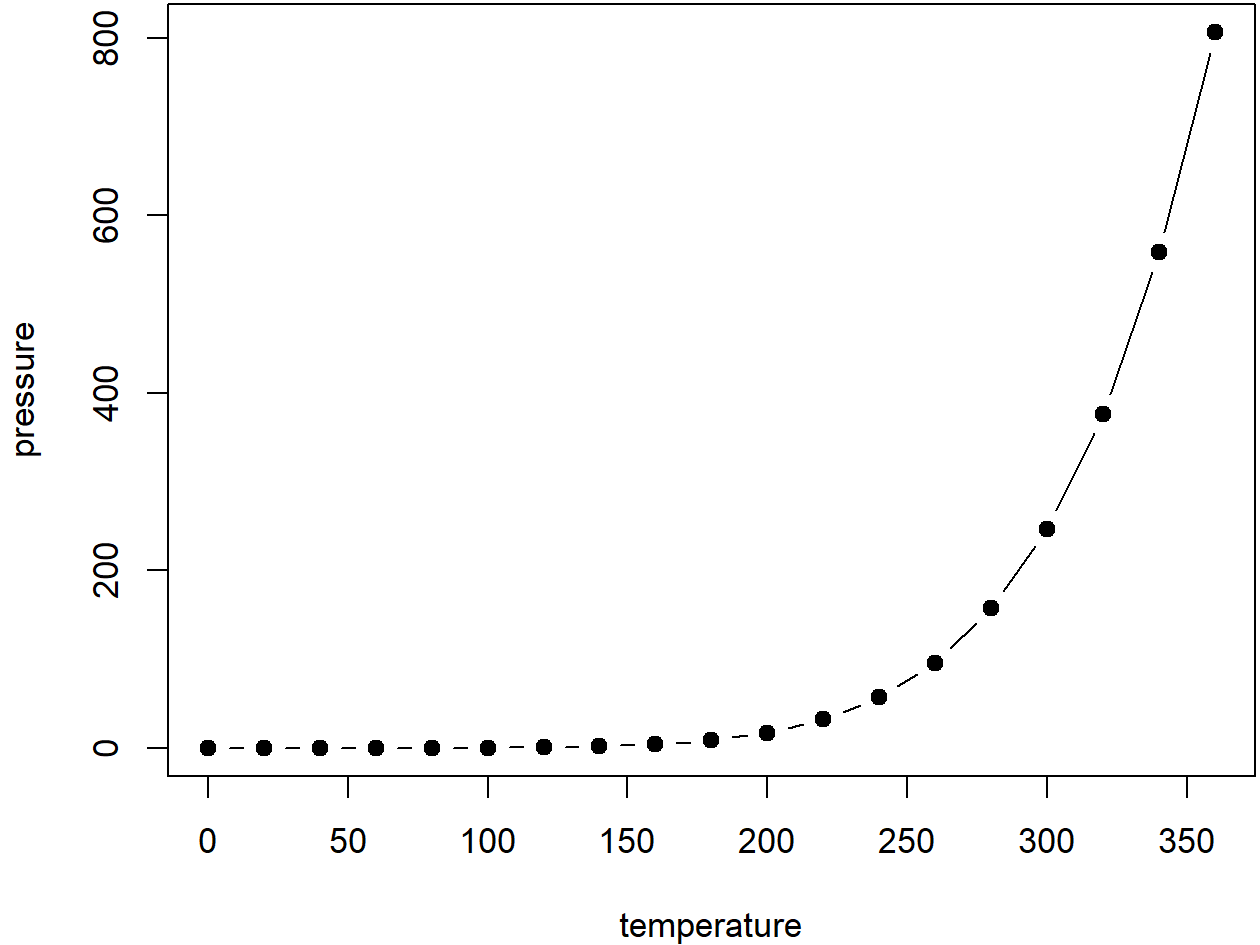
\includegraphics[width=0.8\linewidth]{figures/nice-fig-1} 

}

\caption{Here is a nice figure!}\label{fig:nice-fig}
\end{figure}

Don't miss Table \ref{tab:nice-tab}.

\begin{Shaded}
\begin{Highlighting}[]
\NormalTok{knitr}\SpecialCharTok{::}\FunctionTok{kable}\NormalTok{(}
  \FunctionTok{head}\NormalTok{(pressure, }\DecValTok{10}\NormalTok{), }\AttributeTok{caption =} \StringTok{\textquotesingle{}Here is a nice table!\textquotesingle{}}\NormalTok{,}
  \AttributeTok{booktabs =} \ConstantTok{TRUE}
\NormalTok{)}
\end{Highlighting}
\end{Shaded}

\begin{table}

\caption{\label{tab:nice-tab}Here is a nice table!}
\centering
\begin{tabular}[t]{rr}
\toprule
temperature & pressure\\
\midrule
0 & 0.000\\
20 & 0.001\\
40 & 0.006\\
60 & 0.030\\
80 & 0.090\\
\addlinespace
100 & 0.270\\
120 & 0.750\\
140 & 1.850\\
160 & 4.200\\
180 & 8.800\\
\bottomrule
\end{tabular}
\end{table}

\hypertarget{uxe1mbito-movilidad}{%
\chapter{Ámbito Movilidad}\label{uxe1mbito-movilidad}}

Descripción acá\ldots{}

\hypertarget{instituciones-participantes-2}{%
\section*{Instituciones participantes}\label{instituciones-participantes-2}}
\addcontentsline{toc}{section}{Instituciones participantes}

\emph{Grupo Vialidad e Infraestructura de Transporte}
Dirección de Vialidad - Ministerio de Obras Públicas
Instituto Nacional de Estadísticas
Unidad Operativa de Control de Tránsito - Ministerio de Transportes y Telecomunicaciones
Dirección General de Aeronáutica Civil -- Fuerza Aérea de Chile
Observatorio Urbano -- Ministerio de Vivienda y Urbanismo
Unidad de Pasos Fronterizos -- Ministerio del Interior y Seguridad Pública
División de Desarrollo Logístico - Ministerio de Transporte y Telecomunicaciones\\
Dirección General de Concesiones -- Ministerio de Obras Públicas

\emph{Grupo Transporte Público}
Subsecretaría de Transporte -- Ministerio de Transporte y Telecomunicaciones
Dirección de Transporte Público - Ministerio de Transporte y Telecomunicaciones

\emph{Grupo Accesibilidad}
Consejo Nacional de Desarrollo Urbano
Dirección de Transporte Público - Ministerio de Transporte y Telecomunicaciones
Instituto de Estudios Urbanos UC\\
Cámara Chilena de la Construcción
Subsecretaría de Desarrollo Regional y Administrativo -- Ministerio del Interior y Seguridad Pública
Dirección Nacional de Aduanas

You can add parts to organize one or more book chapters together. Parts can be inserted at the top of an .Rmd file, before the first-level chapter heading in that same file.

Add a numbered part: \texttt{\#\ (PART)\ Act\ one\ \{-\}} (followed by \texttt{\#\ A\ chapter})

Add an unnumbered part: \texttt{\#\ (PART\textbackslash{}*)\ Act\ one\ \{-\}} (followed by \texttt{\#\ A\ chapter})

Add an appendix as a special kind of un-numbered part: \texttt{\#\ (APPENDIX)\ Other\ stuff\ \{-\}} (followed by \texttt{\#\ A\ chapter}). Chapters in an appendix are prepended with letters instead of numbers.

\hypertarget{uxe1mbito-planificaciuxf3n}{%
\chapter{Ámbito Planificación}\label{uxe1mbito-planificaciuxf3n}}

Descripción acá\ldots{}

\hypertarget{instituciones-participantes-3}{%
\section*{Instituciones participantes}\label{instituciones-participantes-3}}
\addcontentsline{toc}{section}{Instituciones participantes}

\emph{Grupo Instrumentos de Planificación Territorial}
Subsecretaría Regional Ministerial - Ministerio de Vivienda y Urbanismo
Centro de Estudio de Ciudad y Territorio -- Ministerio de Vivienda y Urbanismo

\emph{Grupo Usos del Territorio}
Instituto Nacional de Estadísticas
Servicio Nacional de Geología y Minería - Ministerio de Minería
Subsecretaría de Desarrollo Regional y Administrativo -- Ministerio del Interior y Seguridad Pública
Centro de Estudio de Ciudad y Territorio -- Ministerio de Vivienda y Urbanismo
Servicio de Impuestos Internos
Municipalidades
Centro de Información de Recursos Naturales -- Ministerio de Agricultura
Instituto Forestal -- Ministerio de Agricultura
Secretaría Regional Ministerial -- Ministerio de Salud

\emph{Grupo Habitabilidad}
División Técnica de Estudio y fomento Habitacional - Ministerio de Vivienda y Urbanismo
Consejo Nacional de Desarrollo Urbano
Subsecretaria de Desarrollo Regional -- Ministerio del Interior y Seguridad Pública
Superintendencia de Electricidad y Combustible\\
Centro de Estudio de Ciudad y Territorio -- Ministerio de Vivienda y Urbanismo
Instituto Nacional de Estadísticas

\hypertarget{footnotes}{%
\section*{Footnotes}\label{footnotes}}
\addcontentsline{toc}{section}{Footnotes}

Footnotes are put inside the square brackets after a caret \texttt{\^{}{[}{]}}. Like this one \footnote{This is a footnote.}.

\hypertarget{citations}{%
\section*{Citations}\label{citations}}
\addcontentsline{toc}{section}{Citations}

Reference items in your bibliography file(s).

For example, we are using the \textbf{bookdown} package \citep{R-bookdown} (check out the last code chunk in index.Rmd to see how this citation key was added) in this sample book, which was built on top of R Markdown and \textbf{knitr} \citep{xie2015} (this citation was added manually in an external file book.bib).
Note that the \texttt{.bib} files need to be listed in the index.Rmd with the YAML \texttt{bibliography} key.

The RStudio Visual Markdown Editor can also make it easier to insert citations: \url{https://rstudio.github.io/visual-markdown-editing/\#/citations}

\hypertarget{uxe1mbito-riesgos-y-emergencias}{%
\chapter{Ámbito Riesgos y Emergencias}\label{uxe1mbito-riesgos-y-emergencias}}

\hypertarget{instituciones-participantes-4}{%
\section*{Instituciones participantes}\label{instituciones-participantes-4}}
\addcontentsline{toc}{section}{Instituciones participantes}

Descripción acá\ldots{}

\emph{Grupo Amenaza}
Gerencia Protección Contra Incendios Forestales - Corporación Nacional Forestal
Sistema Nacional de Información Territorial -- Ministerio de Bienes Raíces\\
División de Cambio Climático - Ministerio de Medio Ambiente
Servicio Nacional de Geología y Minería - Ministerio de Minería
Subsecretaría Regional Ministerial - Ministerio de Salud

\emph{Grupo Exposición y Vulnerabilidad}
Gerencia Protección Contra Incendios Forestales - Corporación Nacional Forestal
Servicio Nacional de Geología y Minería - Ministerio de Minería\\
Aguas Andinas
Superintendencia de Electricidad y Combustible
Instituto Nacional de Estadísticas\\
Consejo Nacional de Desarrollo Urbano
Registro Civil
Subsecretaría Regional Ministerial de Salud -- Ministerio de Salud\\
Ente Nacional para la Energía Eléctrica\\
División de Cambio Climático - Ministerio del Medio Ambiente

\emph{Grupo Resiliencia}
Corporación Nacional Forestal
Subsecretaría Regional Ministerial - Ministerio del Medio Ambiente
Municipalidades
Oficina Nacional de Emergencia -- Ministerio del Interior y Seguridad Pública

\hypertarget{equations}{%
\section*{Equations}\label{equations}}
\addcontentsline{toc}{section}{Equations}

Here is an equation.

\begin{equation} 
  f\left(k\right) = \binom{n}{k} p^k\left(1-p\right)^{n-k}
  \label{eq:binom}
\end{equation}

You may refer to using \texttt{\textbackslash{}@ref(eq:binom)}, like see Equation \eqref{eq:binom}.

\hypertarget{theorems-and-proofs}{%
\section*{Theorems and proofs}\label{theorems-and-proofs}}
\addcontentsline{toc}{section}{Theorems and proofs}

Labeled theorems can be referenced in text using \texttt{\textbackslash{}@ref(thm:tri)}, for example, check out this smart theorem \ref{thm:tri}.

\begin{theorem}
\protect\hypertarget{thm:tri}{}\label{thm:tri}For a right triangle, if \(c\) denotes the \emph{length} of the hypotenuse
and \(a\) and \(b\) denote the lengths of the \textbf{other} two sides, we have
\[a^2 + b^2 = c^2\]
\end{theorem}

Read more here \url{https://bookdown.org/yihui/bookdown/markdown-extensions-by-bookdown.html}.

\hypertarget{callout-blocks}{%
\section*{Callout blocks}\label{callout-blocks}}
\addcontentsline{toc}{section}{Callout blocks}

The R Markdown Cookbook provides more help on how to use custom blocks to design your own callouts: \url{https://bookdown.org/yihui/rmarkdown-cookbook/custom-blocks.html}

\hypertarget{uxe1mbito-seguridad}{%
\chapter{Ámbito Seguridad}\label{uxe1mbito-seguridad}}

Descripción acá\ldots{}

\hypertarget{instituciones-participantes-5}{%
\section*{Instituciones participantes}\label{instituciones-participantes-5}}
\addcontentsline{toc}{section}{Instituciones participantes}

\emph{Grupo Infraestructura y Equipamiento de Seguridad}
Carabineros de Chile

Unidad Operativa de Control de Tránsito - Ministerio de Transporte y Telecomunicaciones

Junta Nacional de Cuerpos de Bomberos de Chile -- Cuerpo de Bomberos de Chile
Cámara Chilena de la Construcción
Policía de Investigaciones de Chile
Gendarmería
Dirección Nacional de Aduanas
Delegación Presidencial RM
Municipalidades

\emph{Grupo Victimización}
Asociación Chilena de Seguridad
Comisión Nacional de Seguridad de Tránsito - Ministerio de Transporte y Telecomunicaciones
Subsecretaría Regional Ministerial -- Ministerio de Salud
Centro de estudios y Análisis de Delito -- Ministerio del Interior y Seguridad Pública
Carabineros de Chile
Cámara Chilena de la Construcción
Municipalidades

\emph{Grupo Percepción del Delito}
Cámara Chilena de la Construcción
Instituto Nacional de Estadísticas
Centro de estudios y Análisis de Delito - Ministerio del Interior y Seguridad Pública
Subsecretaría de Desarrollo Regional y Administrativo -- Ministerio del Interior y Seguridad Pública

\hypertarget{publishing}{%
\section*{Publishing}\label{publishing}}
\addcontentsline{toc}{section}{Publishing}

HTML books can be published online, see: \url{https://bookdown.org/yihui/bookdown/publishing.html}

\hypertarget{pages}{%
\section*{404 pages}\label{pages}}
\addcontentsline{toc}{section}{404 pages}

By default, users will be directed to a 404 page if they try to access a webpage that cannot be found. If you'd like to customize your 404 page instead of using the default, you may add either a \texttt{\_404.Rmd} or \texttt{\_404.md} file to your project root and use code and/or Markdown syntax.

\hypertarget{metadata-for-sharing}{%
\section*{Metadata for sharing}\label{metadata-for-sharing}}
\addcontentsline{toc}{section}{Metadata for sharing}

Bookdown HTML books will provide HTML metadata for social sharing on platforms like Twitter, Facebook, and LinkedIn, using information you provide in the \texttt{index.Rmd} YAML. To setup, set the \texttt{url} for your book and the path to your \texttt{cover-image} file. Your book's \texttt{title} and \texttt{description} are also used.

\hypertarget{glosario}{%
\chapter*{Glosario}\label{glosario}}
\addcontentsline{toc}{chapter}{Glosario}

\textbf{\texttt{Feature:}} abstracción de un fenómeno del mundo real

\textbf{\texttt{Catálogo\ de\ datos:}} catalogo que contiene definiciones y descripciones de distintos tipos de features, atributos y relaciones entre conjuntos de datos geográficos.

\textbf{\texttt{Ámbito:}} corresponde a la temática principal para agrupar los conjuntos de datos. Se compone de Medio Ambiente, Planificación, Seguridad, Movilidad, Riesgo y Cartografía Base.

\textbf{\texttt{Grupo:}} subcategoría que forma parte de un ámbito, en donde este, puede estar compuesto por dos o más grupos.

\textbf{\texttt{Código\ capa:}} código numérico correlativo de los datos. Se compone de manera jerárquica a partir del tipo de ámbito y grupo en donde se encuentra la información

\textbf{\texttt{Calidad:}} hace referencia al grado de accesibilidad y existencia de la información. Se compone por datos idóneos, los cuales son públicos y accesibles o que los puede proporcionar el GORE; datos suficientes, que se sabe que existen, pero se deben levantar o solicitar a institución pública o privada; y datos insuficientes, que es información que no existe y, por ende, se deberá evaluar la factibilidad para levantar la información.

\textbf{\texttt{Fuente:}} institución pública o privada que elabora la información.

\textbf{\texttt{Documentos\ asociados:}} indica si la información espacial está vinculada legal, administrativa o técnicamente a uno o más documentos. Estos documentos estarán almacenados en un espacio de trabajo por definir.

\textbf{\texttt{Escala\ mínima\ de\ análisis:}} corresponde a la unidad de medida espacial mínima a la cual un dato puede ser trabajado y relacionado con otro tipo de información.

\textbf{\texttt{Cobertura:}} se refiere a la extensión que abarca la información. Pueden ser las siguientes categorías: comunal, provincial o regional.

\textbf{\texttt{Año:}} fecha en la cual se creó la información.

\hypertarget{glosario-del-diagnostico}{%
\section*{Glosario del Diagnostico}\label{glosario-del-diagnostico}}
\addcontentsline{toc}{section}{Glosario del Diagnostico}

\textbf{\texttt{rowname:}} Nombre del columna

\textbf{\texttt{tipo:}} Forma de el variable

\textbf{\texttt{vacios:}} Número de celdas vacías en la columna

\textbf{\texttt{whitespace:}} Número de celdas con solo espacios blancos en la columna

\textbf{\texttt{n\_unico:}} Número de celdas distintas en la columna

\textbf{\texttt{pc\_completo:}} Porcentaje de celdas vacías en la columna

\textbf{\texttt{pc\_repetido:}} Porcentaje de repeticiones

\end{document}
